\section{实验}
\label{sec:experiments}

\subsection{实验设置}
\label{sec:exp-setup}

我们在 StartupBench 上评估 9 个代表性模型，覆盖闭源和开源模型家族：
\begin{itemize}
    \item \textbf{闭源模型：}GPT-5.6-sol~\cite{openai2026gpt56}、GPT-5.5~\cite{openai_gpt55}、Gemini-3.1-Pro~\cite{GoogleCloud2026Gemini3.1Pro}、Seed-2.1-Pro~\cite{bytedance2026seed21}、Qwen-3.6-Max~\cite{qwen36_max_preview}。
    \item \textbf{开源模型：}DeepSeek-V4-Pro~\cite{deepseek2026v4}、Kimi-K3~\cite{team2026kimi}、Kimi-K2.6~\cite{moonshot2026k2_6}、GLM-5.1~\cite{zeng2026glm}。
\end{itemize}
为提高结果的可靠性，我们对每个模型开展 \textbf{3} 次独立运行，并报告任务分数的 95\% bootstrap 置信区间；置信区间通过 10,000 次重采样计算。所有模型均在同一 Nanobot 框架中运行，工具配置完全相同，每项任务的交互步数上限为 \textbf{200}。对每项任务，智能体以任务特定的工作空间和输入请求初始化，其交付物从指定输出目录收集。依照上一节所述评估协议，裁判智能体根据任务说明、工作空间上下文和评分细则集合对这些交付物进行评估。

自动评估所用的裁判智能体也在相同的 Nanobot 框架下运行，以保证执行环境一致，其底层裁判模型为 GPT-5.5。除连续任务分数外，我们还报告\textbf{成功率}，即三次运行合并后成功完成的运行所占比例。若一项任务的最终分数不低于 \textbf{90}，则视为成功；否则计为失败。

\subsection{主要结果}
\label{sec:exp-overall}

\begin{figure}[t]
  \centering
  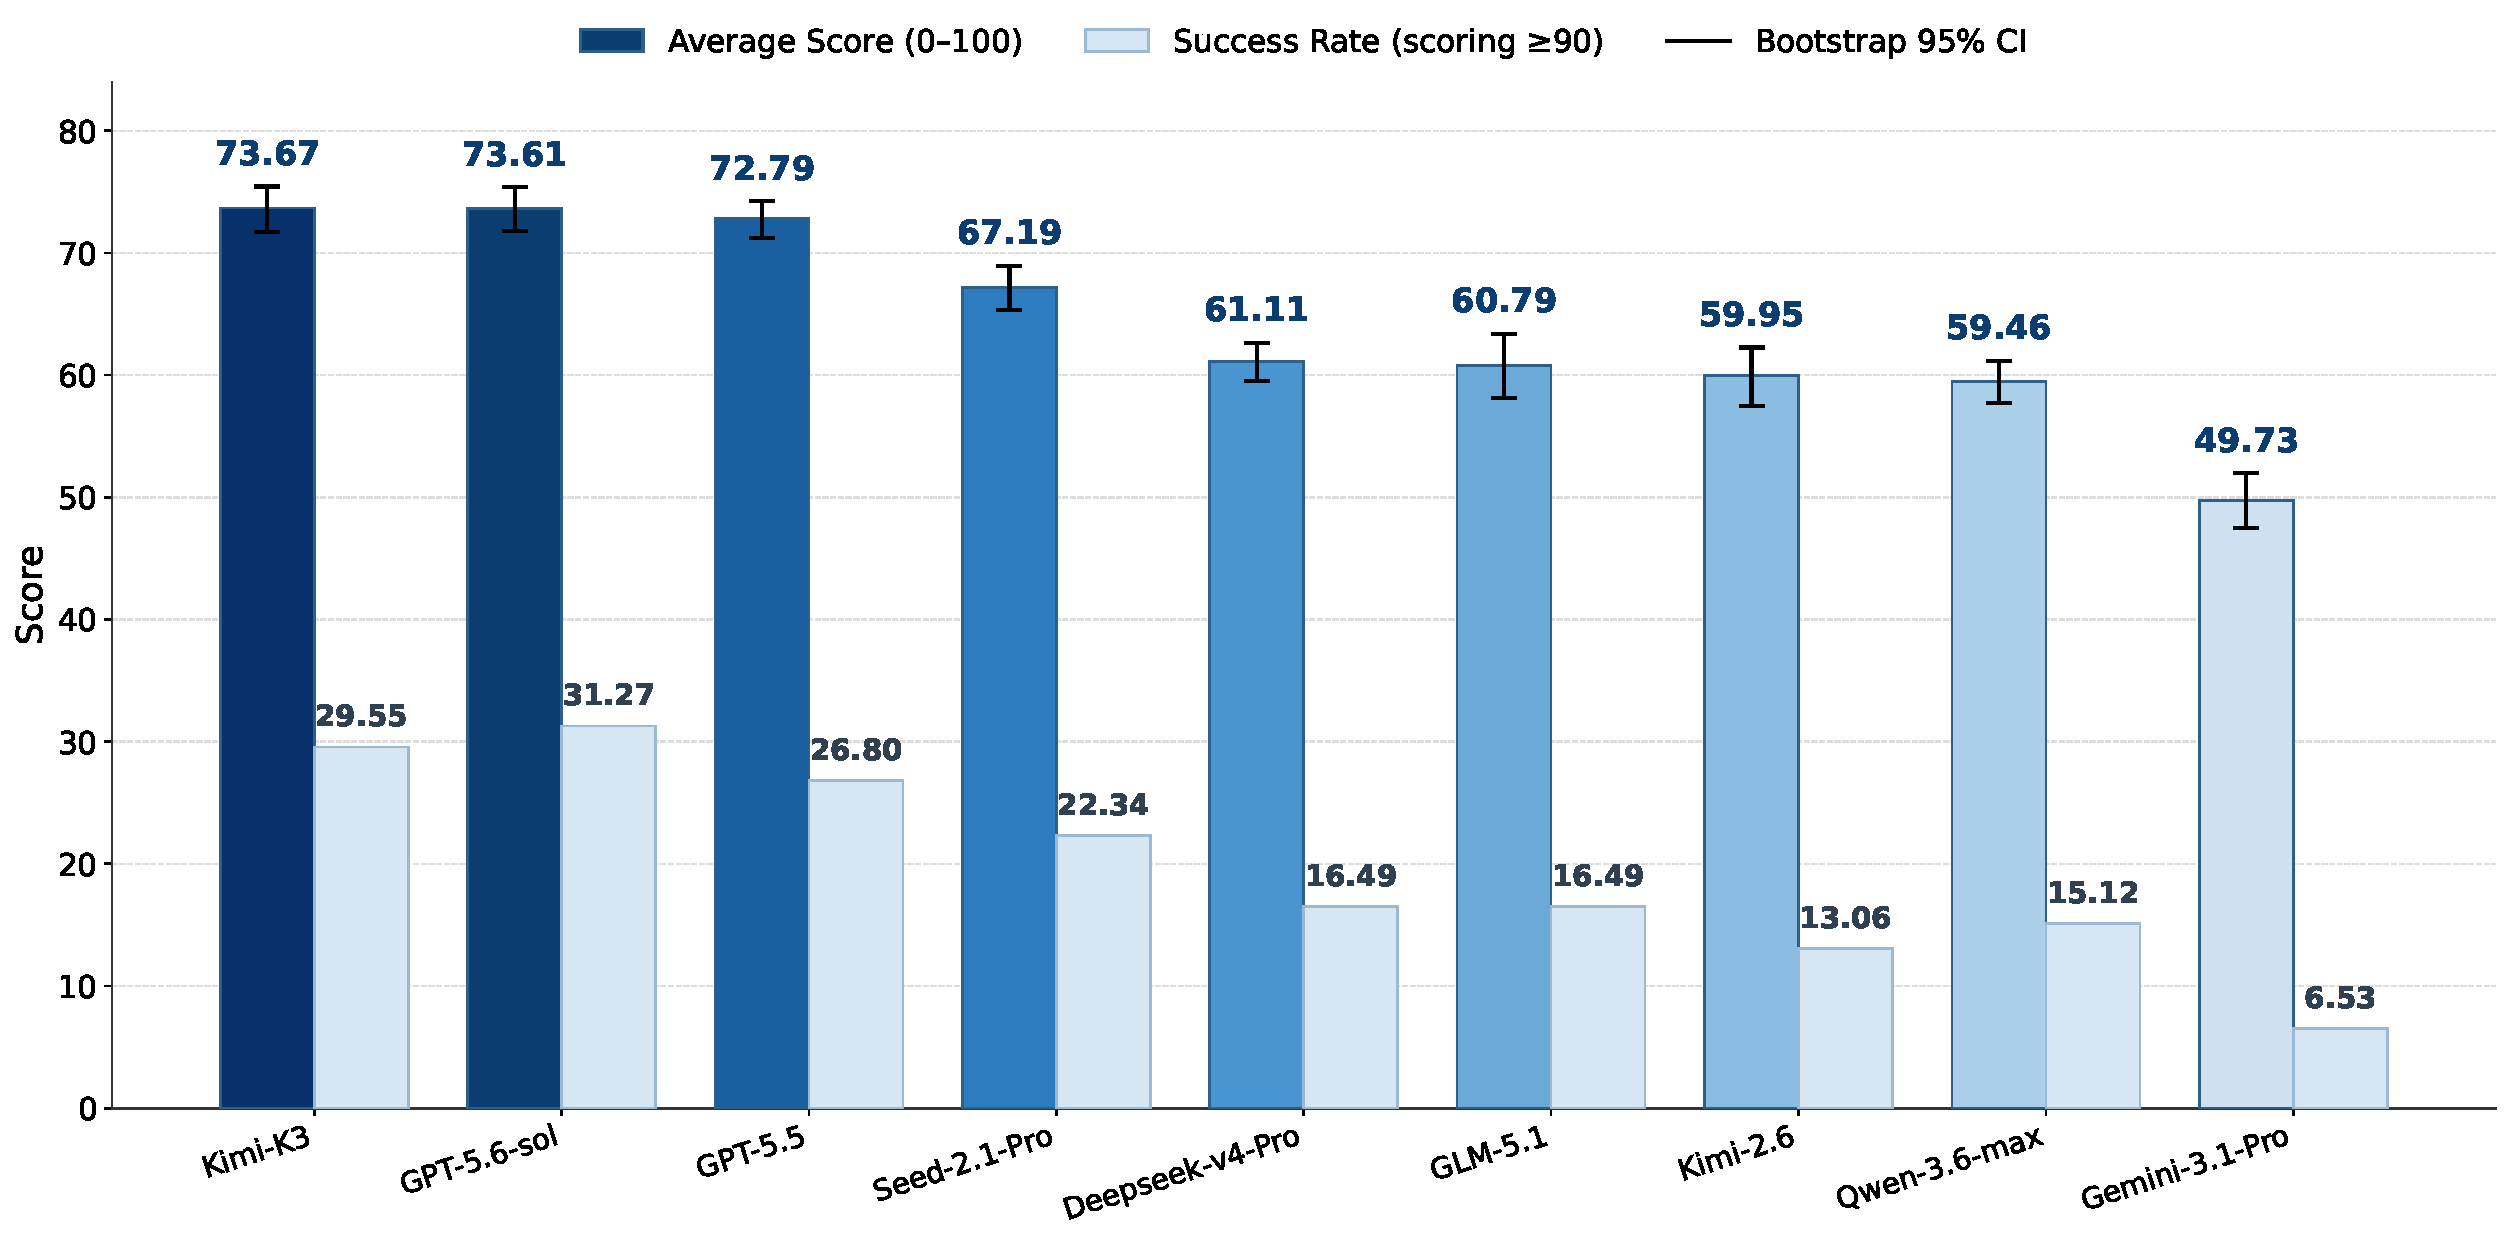
\includegraphics[width=0.95\linewidth]{figures/overall_score_bs_out.pdf}
  \caption{StartupBench 排行榜。}
  \label{fig:overall-leaderboard}
\end{figure}

\begin{table*}[t]
  \centering
  \small
  \setlength{\tabcolsep}{5pt}
  \renewcommand{\arraystretch}{1.15}
  \caption{StartupBench 模型性能，取三次独立运行的平均值。\textbf{上半部分：}按重要性加权的单任务平均分（$0$--$100$）；\textbf{下半部分：}成功率，即三次运行合并后分数 $\ge 90$ 的样本比例（\%）。各列\textbf{最佳值加粗}，\underline{次佳值加下划线}。}
  \label{tab:leaderboard}
  \resizebox{\textwidth}{!}{
  \begin{tabular}{lccccccc}
    \toprule
    \textbf{模型} & \textbf{总体} & \textbf{医疗} & \textbf{金融} & \textbf{法律} & \textbf{商业} & \textbf{STEM} & \textbf{教育} \\
    \midrule
    \multicolumn{8}{c}{\textbf{平均分}} \\
    \midrule
    Kimi-K3 & \textbf{73.67} & \textbf{80.03} & \textbf{62.38} & 69.45 & \textbf{83.90} & 68.34 & \textbf{77.71} \\
    GPT-5.6-sol & \underline{73.61} & \underline{79.32} & 61.66 & \textbf{73.53} & 77.61 & \textbf{74.77} & \underline{73.94} \\
    GPT-5.5         & 72.79 & 78.59 & \underline{62.09} & \underline{71.75} & \underline{79.59} & \underline{72.14} & 68.32 \\
    Seed-2.1-Pro    & 67.19 & 73.15 & 57.26 & 61.35 & 77.83 & 65.61 & 62.91 \\
    Kimi-K2.6       & 59.95 & 67.70 & 51.17 & 54.62 & 71.91 & 51.38 & 58.60 \\
    GLM-5.1         & 60.79 & 65.66 & 51.22 & 50.20 & 78.53 & 52.18 & 66.50 \\
    Qwen-3.6-Max    & 59.46 & 66.51 & 52.45 & 50.33 & 75.03 & 48.83 & 59.26 \\
    DeepSeek-V4-Pro & 61.11 & 69.42 & 51.11 & 54.53 & 73.69 & 54.89 & 57.03 \\
    Gemini-3.1-Pro  & 49.73 & 54.05 & 41.00 & 43.49 & 61.18 & 45.88 & 51.23 \\
    \midrule
    \multicolumn{8}{c}{\textbf{成功率（$\ge90$）}} \\
    \midrule
    Kimi-K3 & \underline{29.55} & \textbf{34.92} & 20.37 & 20.83 & \textbf{52.63} & 16.67 & \underline{23.81} \\
    GPT-5.6-sol & \textbf{31.27} & \underline{33.33} & \textbf{27.78} & \underline{22.92} & 38.60 & \textbf{33.33} & \textbf{28.57} \\
    GPT-5.5         & 26.80 & 30.16 & \underline{22.22} & \textbf{25.00} & 38.60 & \underline{22.92} & 9.52 \\
    Seed-2.1-Pro    & 22.34 & 19.05 & 16.67 & 14.58 & \underline{45.61} & 20.83 & 4.76 \\
    Kimi-K2.6       & 13.06 & 15.87 & 14.81 & 6.25 & 24.56 & 4.17 & 4.76 \\
    GLM-5.1         & 16.49 & 12.70 & 16.67 & 8.33 & 36.84 & 8.33 & 9.52 \\
    Qwen-3.6-Max    & 15.12 & 11.11 & 16.67 & 10.42 & 33.33 & 6.25 & 4.76 \\
    DeepSeek-V4-Pro & 16.49 & 20.63 & 16.67 & 8.33 & 29.82 & 10.42 & 0.00 \\
    Gemini-3.1-Pro  & 6.53 & 6.35 & 11.11 & 6.25 & 8.77 & 0.00 & 4.76 \\
    \bottomrule
  \end{tabular}}
\end{table*}

\textbf{在通用智能体框架下，初创企业任务远未饱和。}尽管最强的 Kimi-K3 和 GPT-5.6-sol 分别取得 73.67\% 和 73.61\% 的平均分，但在严格的验收标准（分数 $\ge 90$）下，没有任何模型能成功完成三分之一的基准任务。更广泛地看，大多数模型的平均分大致位于 55 至 75 之间，说明当前智能体一般能够在解决现实专业工作流方面取得可观进展。然而，高平均分并不必然转化为高任务完成率。Kimi 系列尤其明显：Kimi-K3 的总体平均分最高，但成功率低于 GPT-5.6-sol；类似地，Kimi-K2.6 的平均分高于 Qwen-3.6-Max，成功率却更低。这些差异表明，某些模型虽能满足相当一部分任务要求，却仍无法完整交付。总体而言，所有模型的成功率都明显低于平均分。这说明主要瓶颈已不再是执行工作流的大部分环节，而是能否稳定生成达到直接专业使用标准的产物。

这一差距有两项重要含义。第一，它有助于解释为何专门化垂直智能体仍在许多经过市场验证的工作流中具有实际价值，因为这些场景必须稳定达到专业标准。第二，它说明基础模型的下一个前沿并非只是在执行专业任务，而是可靠地产出无需进一步核验或修改、用户即可采用的工作成果。我们将在第~\ref{sec:exp-failures} 节进一步研究这一差距的根本原因。

\textbf{不同专业领域的性能差异显著。}表~\ref{tab:leaderboard} 表明，当前通用智能体在各种现实工作流中的能力并不均衡。在六个领域中，商业始终最容易：所有模型的平均分都高于 60，跨模型平均成功率也明显高于其他任何领域。相比之下，金融最具挑战，其最低平均分为 54.48\%。商业与金融之间的巨大差距表明，与需要持续定量推理、跨文档一致性和多步核验的工作流相比，当前模型处理结构化程度较高、相对标准化的任务更为可靠。

结果还揭示出显著的领域专长差异。尽管 Kimi-K3 与 GPT-5.6-sol 的总体平均分几乎相同（73.67 对 73.61），两者的强项却大不相同。按成功率看，Kimi-K3 在医疗和商业领域表现最佳，GPT-5.6-sol 在金融、STEM 和教育领域领先，而 GPT-5.5 在法律领域保持最强。平均分也呈现相似格局：Kimi-K3 在医疗、商业、金融和教育领域领先，GPT-5.6-sol 则在法律和 STEM 领域领先。因此，即使在最强模型中，也没有单一智能体能够在所有专业领域始终占优。这些结果说明，当前通用智能体仍存在显著的领域依赖型差异；要提升端到端任务执行在异构专业工作流之间的稳健性和迁移能力，仍有很大改进空间。

\subsection{所提出评估框架的有效性}
\label{sec:exp-agreement}

为验证评估框架的可靠性，我们把它的判断与专家标注进行比较。我们对全部任务抽取两个代表性模型的输出，并请领域专家使用预定义评分细则独立评估每个提交结果。在细则层面，自动评估器与专家判断的总体一致率达到 \textbf{92.78\%}。我们还通过比较最终成功标签，考查这些局部一致是否能转化为一致的任务级决策；当提交结果的聚合分数达到 90 时，即视为成功。自动评估与专家评估在 \textbf{92.84\%} 的成功决策上保持一致。值得注意的是，尽管细则标签和成功标签的分布差异很大，两种层面的高一致率仍非常接近，这表明观察到的一致性并非只是标签不平衡造成的假象。

我们还进一步研究了逐条独立评估评分细则的必要性。在一项消融实验中，我们不再为每条细则分配一个裁判智能体，而是直接把完整模型输出连同全部细则列表交给单个裁判智能体，要求它在一次端到端推理中为所有细则打分。该替代方案使与人类专家的一致率下降到 \textit{83\%}。更重要的是，整体式设置在实践中的稳定性明显更差。裁判智能体必须同时进行长上下文推理、在众多评估标准之间维持一致，并最终生成覆盖所有细则分数的结构化输出，因而经常出现输出格式错误或格式不完整等失败，不得不重复执行。平均而言，每次评估要运行两次以上，才能得到有效结果。相比之下，我们的逐细则评估把考查过程分解为一组相互独立的轻量裁判任务，既明显提升了与人类专家的一致性，也显著改善了执行稳健性。

\subsection{失败模式分析}

\subsubsection{结果层面失败分析}
\label{sec:exp-format}

\begin{figure*}[t]
    \centering
    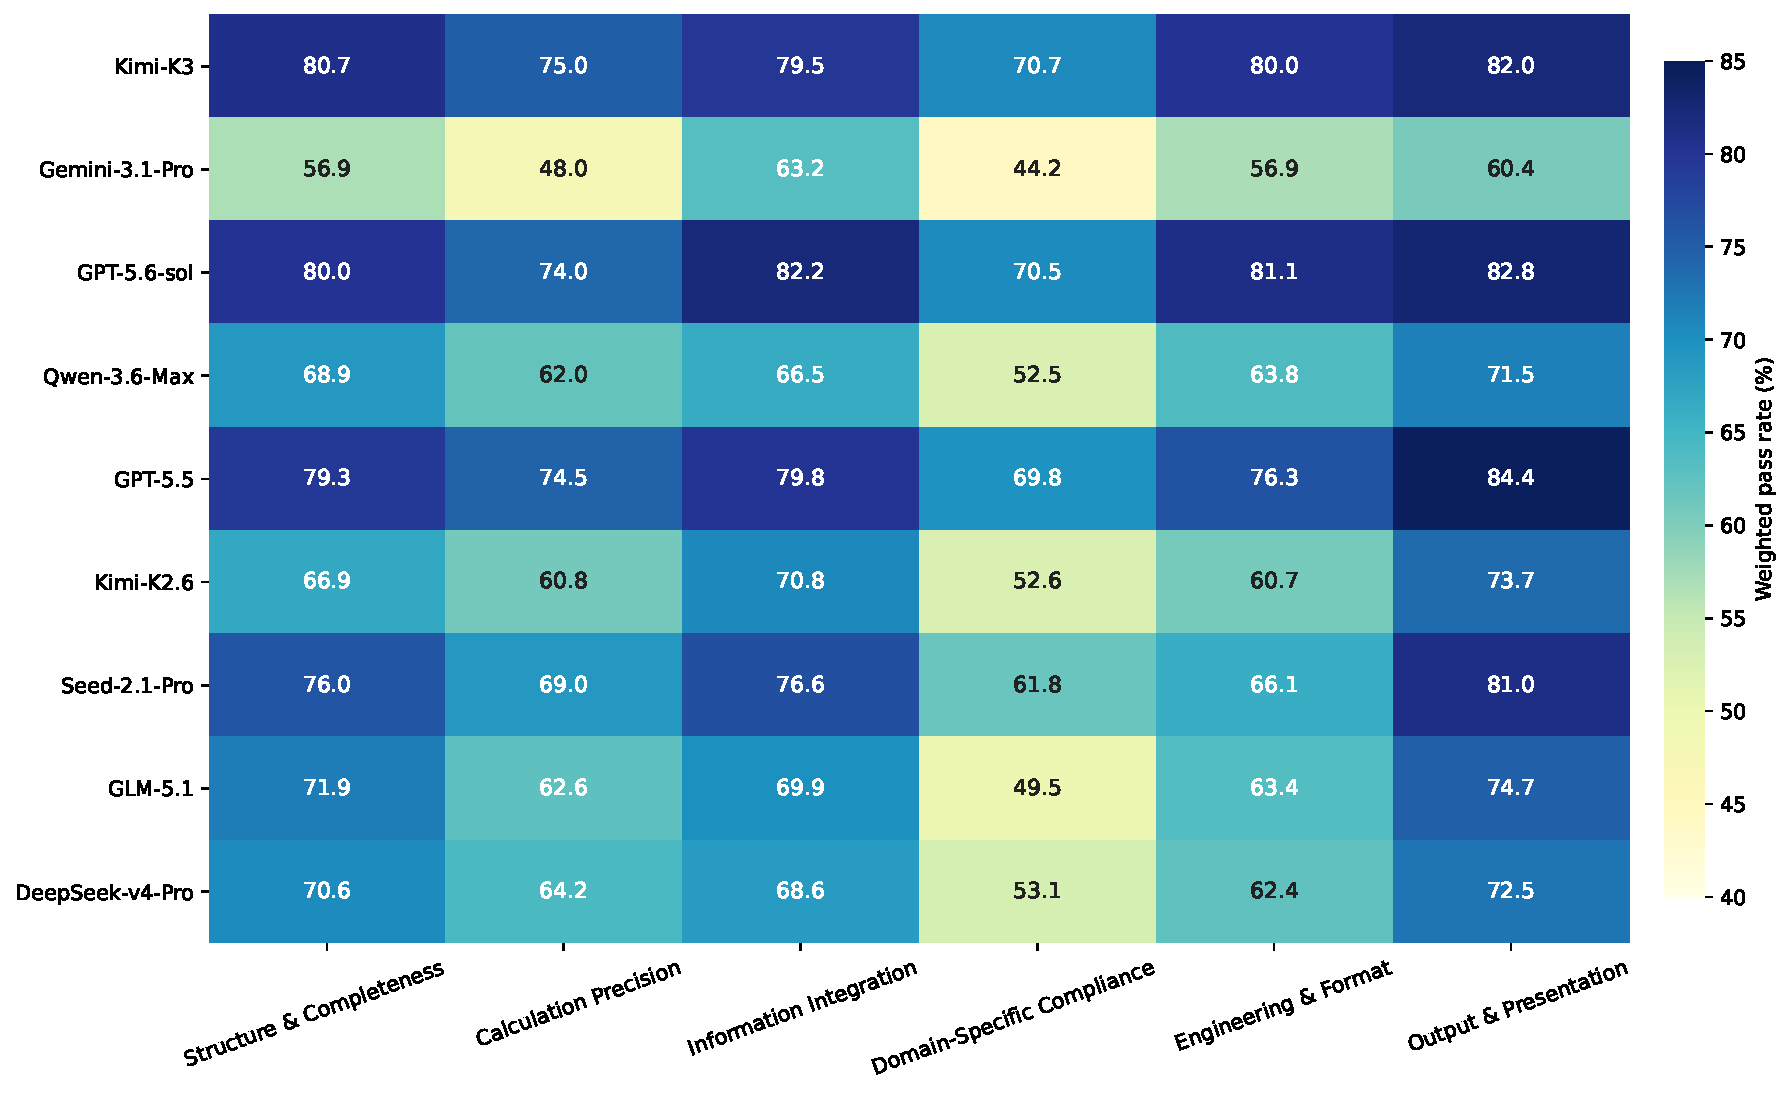
\includegraphics[width=0.99\textwidth]{figures/heatmap_9model.pdf}
    \caption{不同评分细则维度上的表现。图中给出不同模型在 StartupBench 六个评分细则维度上的重要性加权通过率（\%）；数值越高，表示在相应评估维度上的表现越好。}
    \label{fig:dimension-rubric}
\end{figure*}

\textbf{不同评分细则维度上的能力差异。}图~\ref{fig:dimension-rubric} 进一步按评分细则维度拆解模型性能。总体上，当前模型在结构与完整性、信息整合，尤其是输出与呈现维度上始终取得较高分数，说明它们通常能够把异构信息组织成结构良好、视觉上精致的交付物。相比之下，领域特定合规性是所有被评模型最困难的维度，计算精度也明显弱于其他维度。这说明，现代基础模型虽然能生成外观看似完整且专业的产物，但要可靠满足领域特定法规、业务惯例和数值正确性要求，仍是现实部署的一项主要障碍。

最强的两个模型 GPT-5.6-sol 与 Kimi-K3 几乎在所有评分细则维度上都优于其他系统，而非只依赖某一项专门能力。它们最大的优势出现在结构与完整性、计算精度、信息整合和输出与呈现方面，体现出更强的端到端工作流执行和产物构建能力。即便如此，这两个领先模型的最低分仍落在领域特定合规性上，表明遵守专业标准和领域特定要求即使对最先进系统而言仍是首要瓶颈。

\textbf{模型常常满足外围要求，却遗漏最重要的要求。}表~\ref{tab:corefail} 报告了三个重要性层级上经过任务归一化的评分细则满足率。跨模型平均后，满足率从辅助细则的 \textbf{68.67\%} 下降到重要细则的 \textbf{65.89\%}，再降至核心细则的 \textbf{63.45\%}；9 个模型中有 8 个呈现相同的总体趋势。需要强调的是，这些层级反映每项要求对成功完成任务的贡献，而非其预期难度。该模式揭示了当前智能体的一种典型失败：它们往往能够满足辅助性或表层要求，却会在决定任务能否真正成功完成的核心要求上失手。换言之，明显的表面进展可能来自完成任务中不太关键的部分，而关键遗漏仍会使最终交付物无法实际使用。

图~\ref{fig:corefail} 展示了模型难以满足任务完成核心要求的典型案例。在这项机械工艺任务中，模型经常完成工作簿的外围要求，却未能完成核心技术操作：从工程图中准确提取尺寸、根据所给文档核验规格，以及把发现的差异与相应整改措施关联起来。即使许多辅助要求已经完成，这些失败仍使所得工作簿无法实现其主要用途。

\begin{table}[t]
\centering
\small
\caption{不同重要性层级上经过任务归一化的评分细则满足率（\%）。对每个模型--任务--试验组合，我们先计算各重要性层级内的满足率，再在任务和试验之间求平均。}
\label{tab:corefail}
\resizebox{\linewidth}{!}{
\begin{tabular}{lccc}
\toprule
\textbf{模型} & \textbf{辅助} & \textbf{重要} & \textbf{核心} \\
\midrule
Kimi-K3          & 77.89 & 75.12 & 73.40 \\
GPT-5.6-sol      & 77.59 & 74.47 & 73.07 \\
GPT-5.5          & 75.12 & 75.09 & 72.07 \\
Seed-2.1-Pro     & 70.83 & 69.85 & 65.77 \\
Kimi-K2.6        & 66.64 & 63.56 & 57.82 \\
GLM-5.1          & 64.58 & 61.40 & 60.68 \\
Qwen-3.6-Max     & 65.39 & 62.17 & 58.08 \\
DeepSeek-V4-Pro  & 66.50 & 62.97 & 60.05 \\
Gemini-3.1-Pro   & 53.48 & 48.41 & 50.13 \\
\midrule
\textbf{平均} & \textbf{68.67} & \textbf{65.89} & \textbf{63.45} \\
\bottomrule
\end{tabular}}
\end{table}

\begin{figure*}[t]
    \centering
    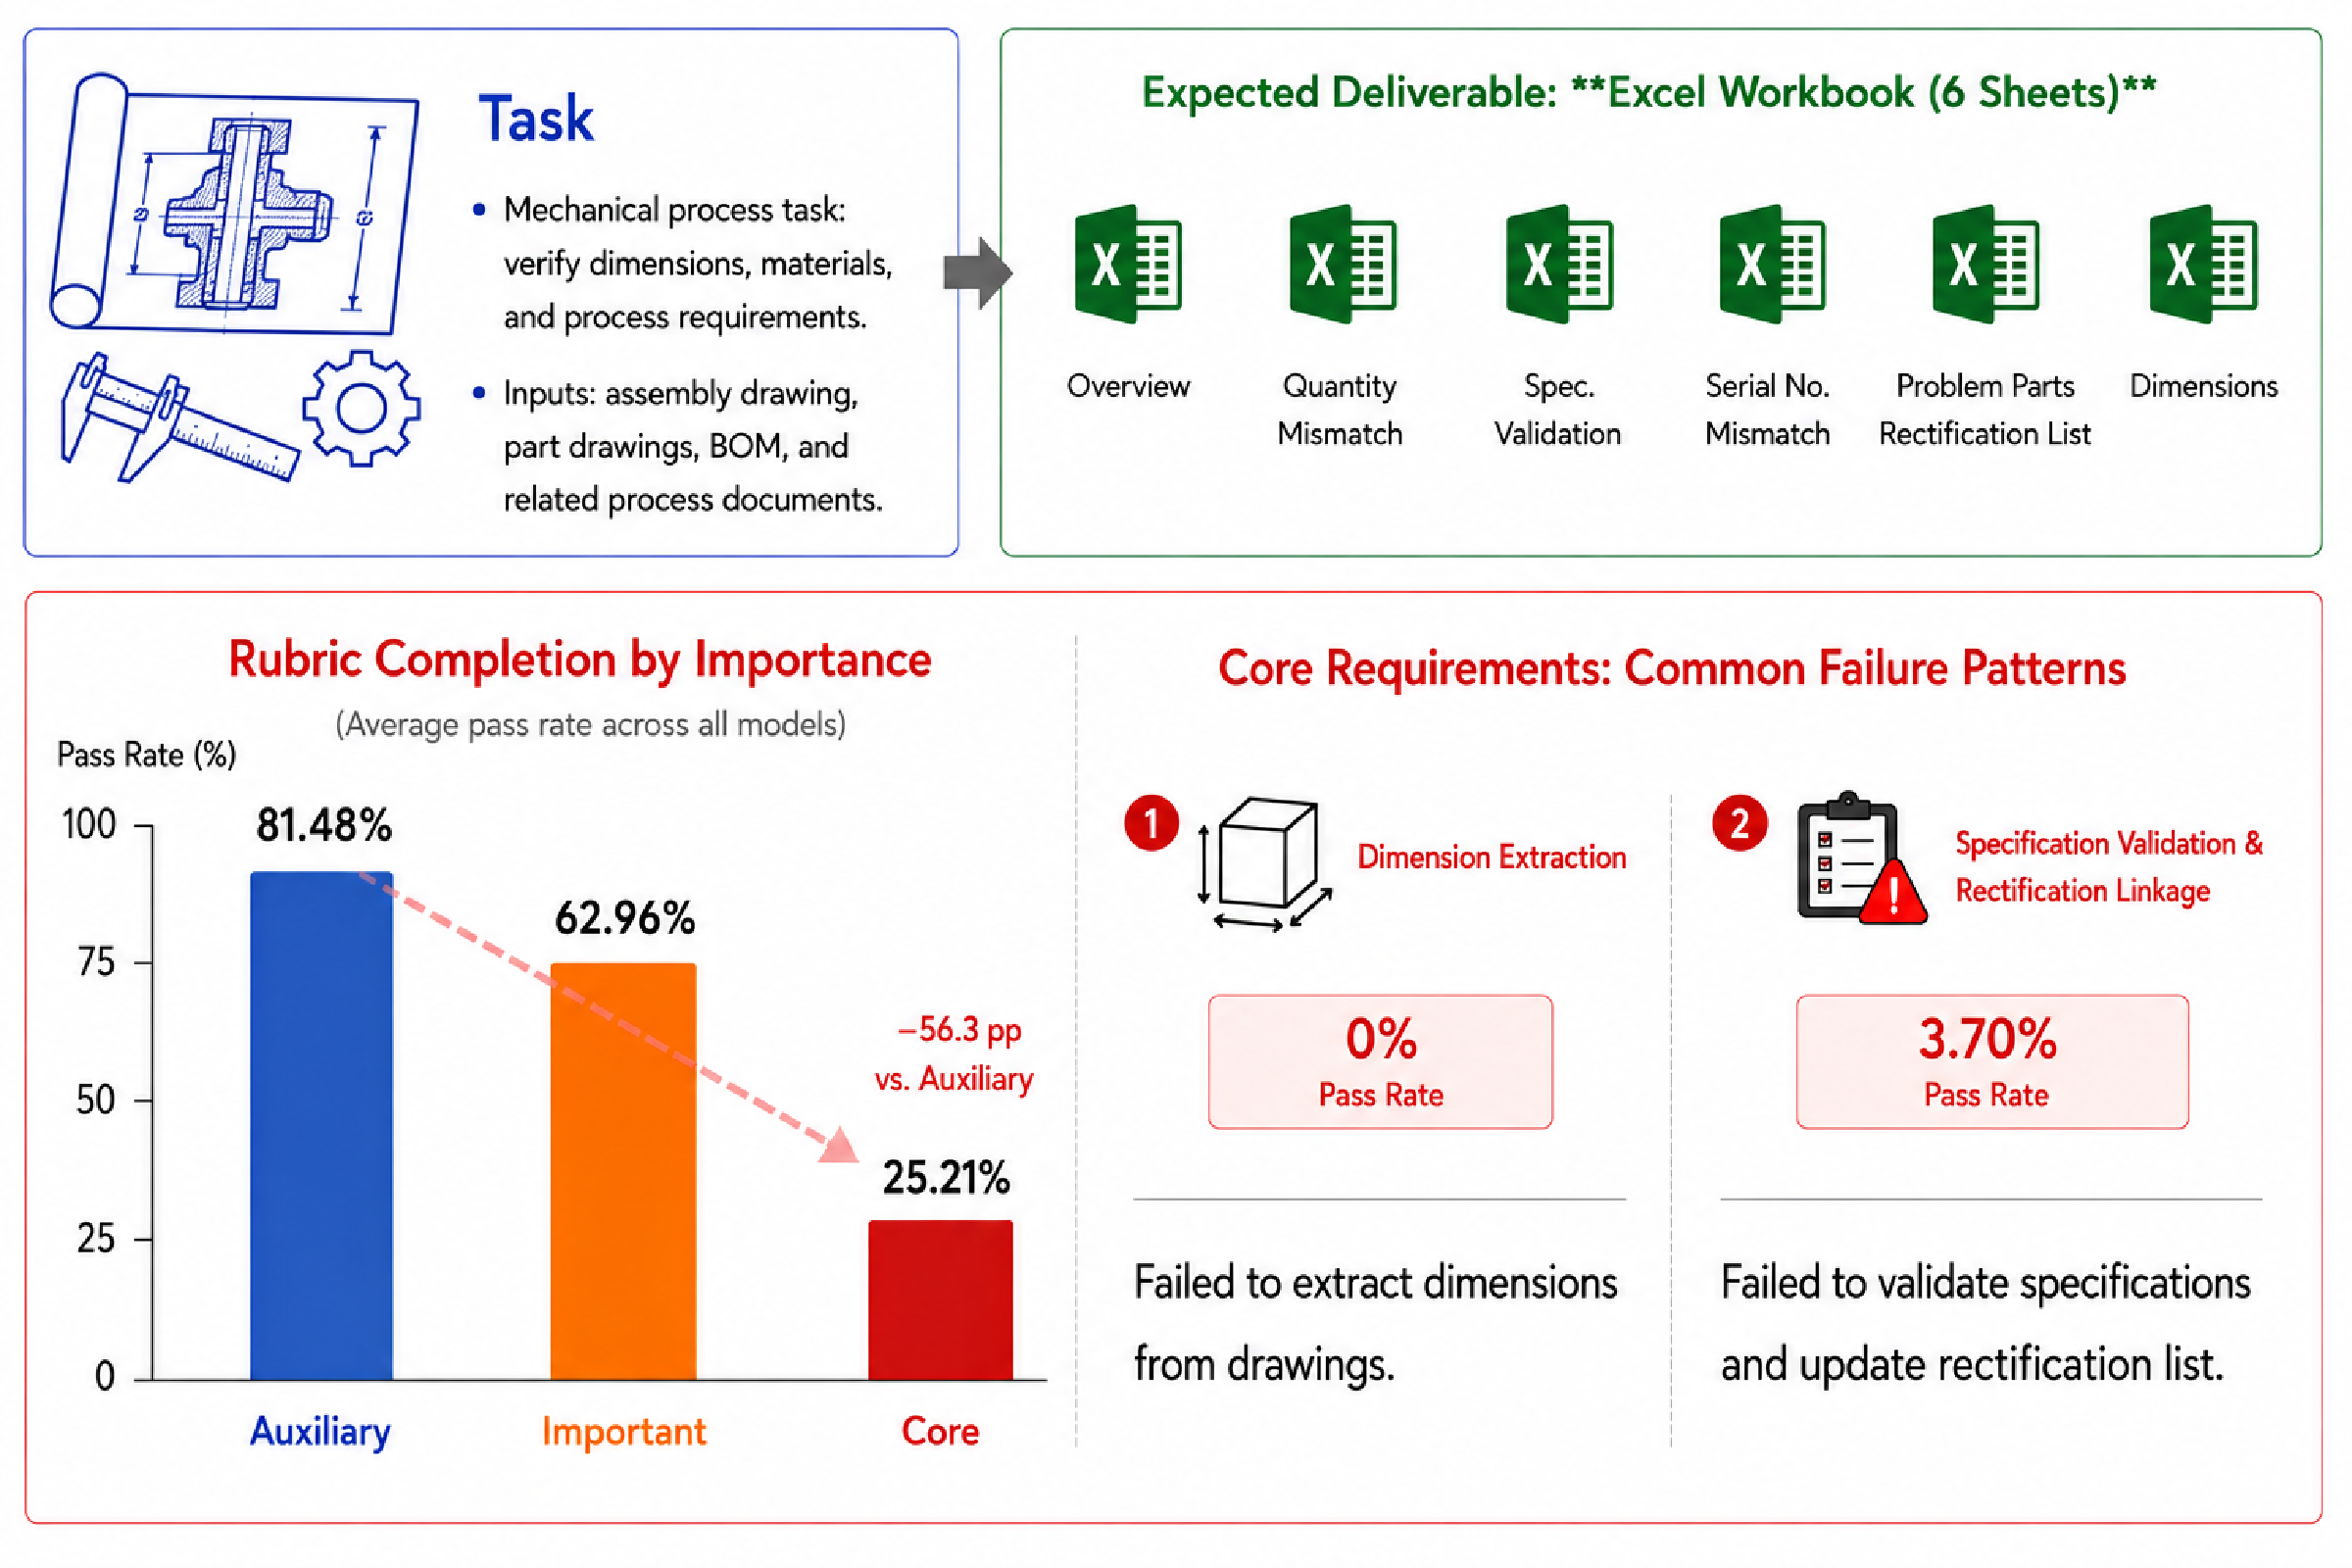
\includegraphics[width=0.8\textwidth]{figures/rubric_corefail_case.pdf}
    \caption{StartupBench 中模型未通过核心评分细则、却通过辅助评分细则的一个代表性案例。}
    \label{fig:corefail}
\end{figure*}

\textbf{输出格式不合规。}部分失败源于模型没有使用任务明确要求的文件类型生成交付物。与前文讨论的大多数失败模式不同，这项要求既不涉及复杂推理，也不需要领域知识，而且可以根据文件扩展名确定性地验证。尽管如此，在 56 项明确规定输出格式的任务上，没有任何模型达到完全合规（表~\ref{tab:format-compliance}），合规率介于 $97.6\%$ 与 $86.3\%$ 之间。大多数违规可归入两种反复出现的模式：生成错误的文件类型（例如以 \texttt{.md}/\texttt{.txt} 代替要求的 \texttt{.pdf}），以及遗漏部分请求的交付物（例如要求同时生成 \texttt{.xlsx} 和 \texttt{.docx}，却只生成其中一种）。这些错误表明，即使是基本的交付物层面约束，对当前基础模型而言仍是不可忽视的失败来源。

\begin{table}[t]
\centering
\footnotesize
\caption{56 项含明确输出文件要求细则的 StartupBench 任务上的输出格式合规率。模型按合规率排序。}
\label{tab:format-compliance}
\begin{tabular}{lc}
\toprule
\textbf{模型} & \textbf{合规率（\%）}\\
\midrule
Kimi-K3           & 97.6 \\
Seed-2.1-Pro      & 95.2 \\
GPT-5.6-sol       & 94.6 \\
Qwen-3.6-Max      & 94.6 \\
DeepSeek-V4-Pro   & 94.0 \\
GPT-5.5           & 93.5 \\
Kimi-K2.6         & 92.9 \\
Gemini-3.1-Pro    & 86.9 \\
GLM-5.1           & 86.3 \\
\bottomrule
\end{tabular}
\end{table}

\subsubsection{行为层面失败分析}
\label{sec:exp-failures}

\textbf{复杂指令遵循。}复杂的现实工作流通常会对最终交付物提出大量约束，包括结构组织、计算逻辑、格式和可执行正确性。尽管任务描述明确列出这些要求，当前模型仍经常只做到部分合规：它们满足最显眼的要求，却忽略其他同样关键的约束。因此，生成的产物经粗略检查似乎大体完整，却不满足直接使用所需的全部验收标准。该行为表明，模型往往在优化“看起来正确”的输出，而非确保每一条支配最终交付物的指令都得到忠实执行。

图~\ref{fig:instruction} 展示了一个代表性案例。该任务要求根据多个源工作表生成完整的人力资源薪资工作簿，并满足多种结构、计算和格式约束。尽管模型生成的产物看起来大体完整，包括所有要求的工作表、公式、图表和仪表板布局，产物层面评估却发现仍有若干关键验收条件未满足。具体而言，下游验证所需的关键缓存值缺失，使这个外观精致的工作簿无法核验。该案例体现了常见的部分合规模式：模型满足最显眼的要求，却忽略不那么明显但同样不可或缺的交付物约束。

\begin{figure*}[t]
    \centering
    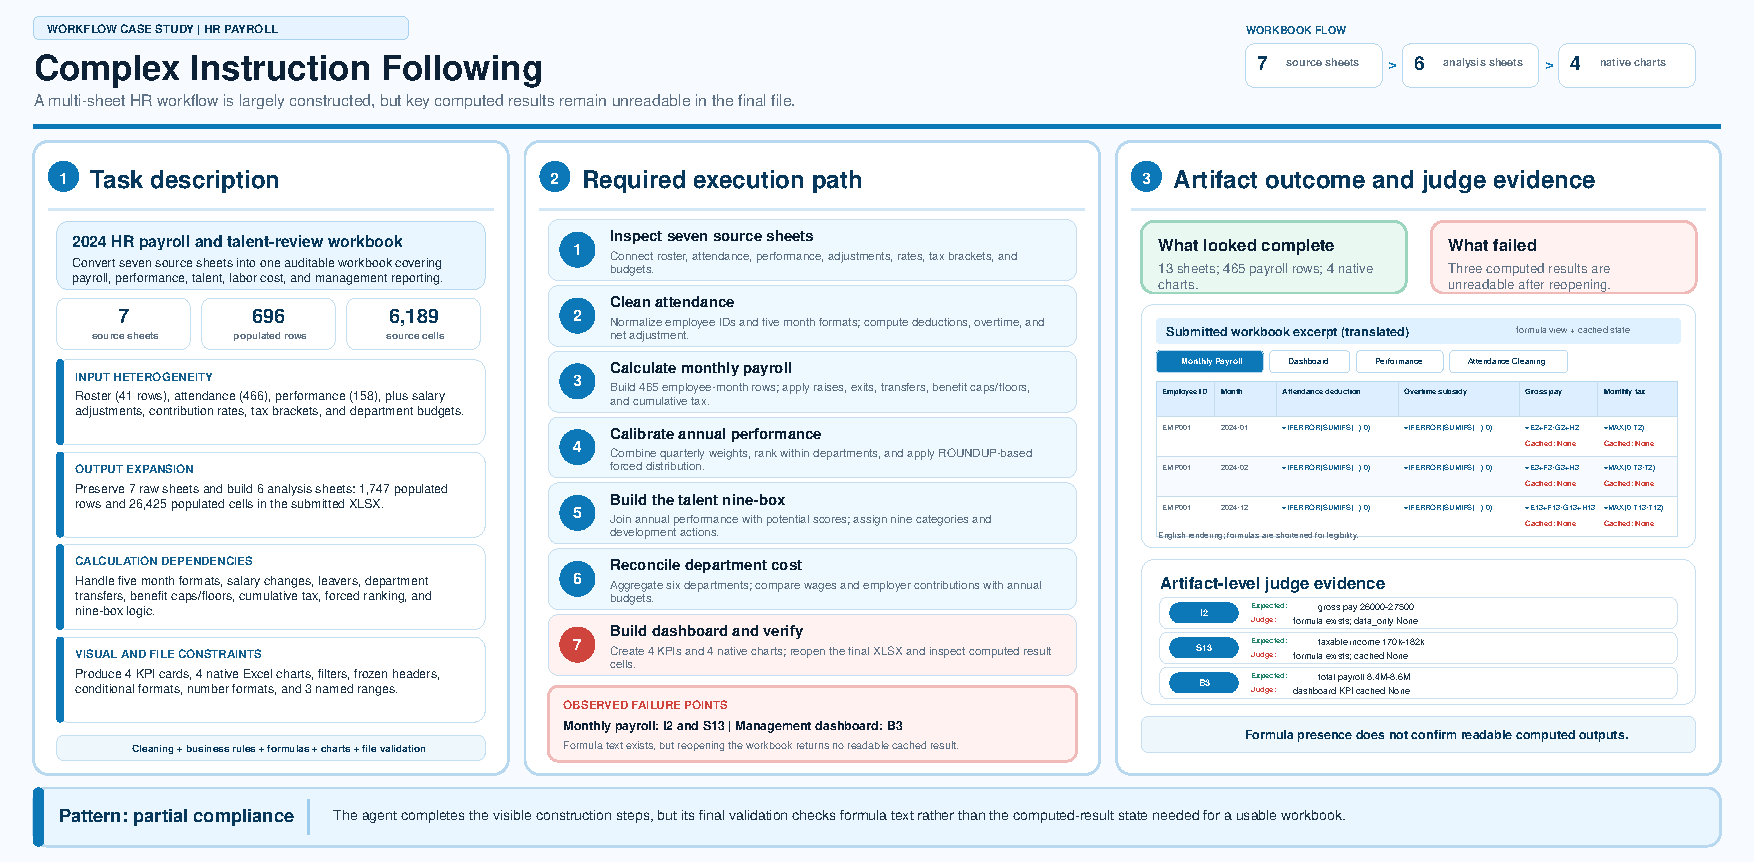
\includegraphics[width=0.99\textwidth]{figures/figure5_hr.pdf}
    \caption{复杂指令遵循失败的一个代表性案例。尽管生成的工作簿看似完整，产物层面评估仍发现多个关键验收条件未满足，体现了常见的部分合规模式。}
    \label{fig:instruction}
\end{figure*}

\textbf{自我验证幻觉。}我们还观察到，许多模型失败并非因为无法完成所需工作流，而是因为它们错误地假定“执行成功”等同于“交付成功”。模型在生成一个看似合理的产物后，常把预期的推理过程或已执行步骤总结为任务已经通过验证的证据，却不依据原始用户要求独立检查最终交付物。于是，单元格数值错误、标识符无法匹配、约束缺失或格式不一致等细微但关键的问题，即使在一个看似可信的输出中也不会被发现。该行为体现了一种自我验证幻觉：模型把对自身推理过程的信心误当成生成产物满足验收标准的证据。然而在现实办公工作流中，成功完成任务要求验证最终交付物本身，而不是只确认执行过程；因此，这种幻觉是部署关键型失败的常见来源。典型案例见附录~\ref{app:self-verify hallucination}。

\textbf{领域专门知识。}另一个主要失败来源是领域专门知识不足，这与领域特定合规性维度上相对较差的表现一致。与通用指令遵循错误不同，这些失败由不同专业领域独特的操作要求造成。模型往往能生成措辞流畅、格式专业的输出，却经常不能满足决定交付物是否真正可用的领域特定约束。因此，主要失败模式因领域而有显著差异，反映出现实工作流对正确性、证据、精度和可操作性的不同要求。

从领域视角看，不同专业领域暴露出各异的失败特征。商业与管理任务主要考验产物正确性，特别是电子表格、仪表板、公式和结构化报告。金融任务强调来源归因、数值精度、估值假设和时间一致性，错误通常来自核对不足、数值自检不充分或会计惯例不一致。法律任务受到法律文书风格的约束相对较少，更受法律推理完整性和正确性的限制，包括引用缺失、事实覆盖不全、成文法依据不足，或事实与适用规则映射错误。医疗任务的平均分相对较高，但安全风险明显更大，因为用药时机、继续治疗标准或出院规划方面的错误会直接破坏临床可用性。STEM 与计算机科学任务则要求精确的对象层面落地，即准确把握代码、工程图、图像、物料清单和系统组件之间的关系。最后，教育与人文学科任务更强调细粒度规则遵循，例如课程要求、学分分配、文档组织和文本连贯性。领域专门知识不足所致失败的一个典型示例见附录~\ref{app:domain}。

\subsection{智能体框架对初创企业任务的影响}

\subsubsection{通用智能体框架的影响}
\begin{table}[t]
\centering
\small
\renewcommand{\arraystretch}{1.15}
\caption{不同通用智能体框架下的性能。对每个模型，我们报告三个通用框架下的平均分，以及框架间性能极差（最大值减最小值）。}
\label{tab:harness}
\resizebox{\linewidth}{!}{
\begin{tabular}{lcccc}
\toprule
\textbf{模型} & \textbf{Hermes} & \textbf{Claude Code} & \textbf{Nanobot} & \textbf{极差} \\
\midrule
GPT-5.5  & 71.00 & 70.11 & 72.79 & 2.68 \\
GLM-5.1  & 60.20 & 60.18 & 60.79 & 0.61 \\
Qwen-3.6-Max & 59.10 & 57.38 & 59.46 & 2.08 \\
\midrule
平均  & 63.43 & 62.56 & 64.35 & 1.79 \\
\bottomrule
\end{tabular}}
\end{table}

在主实验中，所有模型都在 Nanobot 智能体框架下评估。为考查观察到的性能是否主要由智能体框架选择而非底层模型决定，我们使用另外两个代表性通用智能体框架 Hermes~\cite{hermes_agent} 和 Claude Code~\cite{anthropic_claude_code} 重新评估基准。所有框架均使用相同任务集和完全相同的评估协议，只有执行框架被替换。

如表~\ref{tab:harness} 所示，更换通用框架只会造成很小的性能差异。在所有被评模型中，最佳与最差框架之间的平均差异仅为 1.79 分。GLM-5.1 几乎完全不受影响（0.61 分），即使 GPT-5.5 上观察到的最大差异也只有 2.68 分。更重要的是，三个框架下模型的相对排序保持不变。这些结果表明，StartupBench 基本不受通用智能体框架选择的影响。尽管不同框架采用不同的提示策略、工具接口和交互机制，单纯替换通用框架并不会显著改变端到端任务性能。因此，StartupBench 上观察到的性能差距主要反映底层基础模型的能力，而非某个特定框架的实现特征。

\subsubsection{通用智能体与专门化智能体}
为进一步理解智能体框架的作用，我们把通用智能体框架与 StartupBench 任务所源自的专门化初创企业智能体进行比较。与上一实验不同，这项比较对每个任务使用相应的生产级初创企业智能体；这些智能体已通过领域特定模型选择、提示策略、工具编排和工作流设计，针对其目标工作流进行专门优化。

表~\ref{tab:general_specialized} 汇总了通用与专门化智能体系统的比较。综合全部执行，通用智能体的平均分为 64.26，成功率为 19.74\%，明显低于专门化智能体的 83.50 和 39.18\%。由于专门化智能体明确针对目标领域进行设计和优化，我们还为通用智能体考虑了一个更强的 oracle 设置：对每个模型--任务组合，保留三次独立试验中的最佳结果。该 oracle 选择把平均分提高到 71.75、成功率提高到 28.06\%，但仍明显落后于专门化智能体；平均分相差 11.75 分，成功率相差 11.12 个百分点。因此，这一性能差距不能只用随机变化或偶发执行失败来解释：即使允许通用智能体多次尝试并按观测到的最佳结果评估，专门化智能体系统在这些任务上仍明显更有效。

结合前述失败模式分析，这些发现更完整地刻画了通用基础模型与专门化初创企业智能体之间尚存的差距。尽管当今基础模型在统一通用框架下仍无法完全取代领域专门化智能体，其短板集中在一组相对明确的能力上，包括复杂指令遵循、领域特定知识、专业操作惯例和长时程工作流执行。这表明，专门化系统目前观察到的优势未必需要根本不同的智能体架构，而可能反映当前通用模型尚未可靠掌握的能力。随着这些底层能力继续改进，通用智能体或将越来越多地完成有价值的专业端到端任务，而无需依赖领域特定的智能体框架设计。

\begin{table}[t]
\centering
\small
\caption{通用智能体系统与专门化智能体系统的比较。Oracle General 表示对每个模型的全部试验取最高分后所得平均值。}
\label{tab:general_specialized}
\begin{tabular}{lcc}
\toprule
\textbf{智能体系统} & \textbf{平均分} & \textbf{成功率} \\
\midrule
通用（全部运行平均） & 64.26 & 19.74 \\
通用（Oracle） & 71.75 & 28.06 \\
专门化智能体 & \textbf{83.50} & \textbf{39.18} \\
\bottomrule
\end{tabular}
\end{table}

\onecolumn
\noindent\begin{minipage}[t]{0.48\textwidth}
\section{结论}
我们提出 \textbf{StartupBench}，用于评估模型在源自经过市场验证的人工智能原生产品和现实用户需求的端到端专业工作流上的表现。我们对跨越多个领域的多项任务开展评估，揭示了“在专业工作上取得有意义的进展”与“生成完全满足实际验收标准的交付物”之间的显著差距。该差距主要由复杂指令遵循、领域专门知识、专业惯例和长时程工作流执行方面的局限造成。通过把评估植根于用户已经希望委派给人工智能的工作流，StartupBench 为衡量智能体的实际能力提供了一项现实尺度，并指出未来改进的具体方向。我们希望 StartupBench 能支持模型和智能体的发展，使其不仅能够完成有价值的专业工作，还能可靠地交付可供直接使用的结果。

\end{minipage}\hfill
\begin{minipage}[t]{0.48\textwidth}
\section{贡献}

\textbf{项目负责人} \\
Liya Zhu, Xin Ma, Tao Liu, Haodong Wang, Ge Zhang \\

\vspace{0.5em}
\textbf{核心贡献者} \\
Jingzhe Ding, Qingshui Gu, Yongjie Zhong, Jinxiang Meng, Yuan Gao,
Yunqiu Zhou, Hao Zhu, Jifeng He,
Yongzhi Liao, Xinyi Zhang, Chaoxin Li, Yi Zhu,
Xi Lin, Duju Zeng, Xiang Gao, Wen Zhang,
Yunyang Wang, Duo Wang \\

\vspace{0.5em}
\textbf{贡献者} \\
Huan Zhou, Zuo Wang, Jin Chen, Kaiyuan Zhang, Chuqian Yu, Tianhao Yu, Longxiang Liu, Jianbo Xue, Huimin Che, Jiahao Wang \\

\vspace{0.5em}
\textbf{资助委员会} \\
Yujia Qin, Jiaheng Liu

\vspace{0.5em}
\textbf{通讯作者} \\
Ge Zhang (\email{gezhang@umich.edu})\\
Shen Yan (\email{sheny@bytedance.com}) \\
Xiaolong Chang (\email{changxiaolong@bytedance.com})\\
Wenhao Huang (\email{huang.wenhao@bytedance.com})\\
\end{minipage}
\twocolumn
